\chapter{Stos protokołów LTE}
\label{cha:protokoly}

Do prawidłowej komunikacji pomiędzy poszczególnymi urządzeniami w sieci najczęściej potrzebny jest zestaw wielu mechanizmów i reguł, które uczynią ją możliwą a także efektywną. Aby zmniejszyć ich złożoność a także ułatwić zrozumienie, implementację i dalszy rozwój takie mechanizmy i reguły są dzielone na osobne protokoły stanowiące razem stos protokołów. W stosie protokołów protokoły najniższego rzędu odpowiadają za komunikację ze sprzętem a protokoły najwyższego rzędu udostępniają interfejs z którego korzystają aplikacje przestrzeni użytkownika. Pomiędzy nimi znajdują się pośrednie warstwy dodające funkcjonalności takie jak korekcja błędów, kompresja, zapewnienie kolejności, eliminacja duplikatów.

Protokoły tego samego rzędu na jednym urządzeniu wymieniają komunikaty pomiędzy protokołem tego samego rzędu na sąsiednim urządzeniu (strzałka 1. na Rys. \ref{fig:protocols_stack}). Podczas wysyłania danych protokoły wyższego rzędu wysyłają komunikaty do protokołów niższego rzędu (strzałka 2. na Rys. \ref{fig:protocols_stack}) a podczas odbierania danych protokoły niższego rzędu wysyłają komunikaty do protokołów wyższego rzędu (strzałka 3. na Rys. \ref{fig:protocols_stack}). 

\begin{figure}
	\centerline{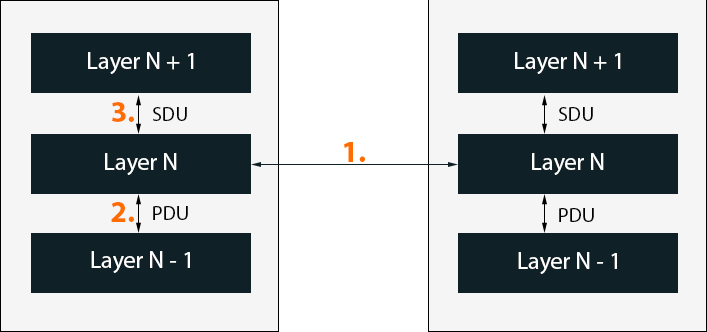
\includegraphics[width=0.6\textwidth]{images/protocols.png}}
	\caption{Ogólny model stosu protokołów}
	\label{fig:protocols_stack}
\end{figure}

Przez protokół określamy szczegóły implementacyjne danej warstwy tj. mechanizmy i reguły zaimplementowane w jej obrębie. Natomiast jako serwis nazywamy interfejsy, które dana warstwa udostępnia warstwom sąsiadującym. \cite{Ahm13} Dane otrzymywane przez daną warstwę z warstwy wyższej określamy jako Service Data Unit (SDU) natomiast dane wysyłane przez daną warstwę do warstw niższych jako Protocol Data Unit (PDU). 
Tak więc przy transmisji danych warstwa N odbiera SDU z warstwy N + 1 i wysyła PDU zawierające przetworzone SDU z dodanymi nagłówkami do warstwy N - 1. Natomiast podczas odbierania danych warstwa N odbiera PDU z warstwy N - 1 i wydobywa z niej SDU, które wysyła do warstwy N + 1. Warto również zauważyć, że jednostka danych, która z punktu widzenia warstwy N jest określana jako SDU z punktu widzenia warstwy N + 1 jest określana jako PDU. I tak samo jednostka danych, która z punktu widzenia warstwy N jest określana jako PDU z punktu widzenia warstwy N - 1 będzie określana jako SDU.

\section{Model OSI}

\begin{figure}
	\centerline{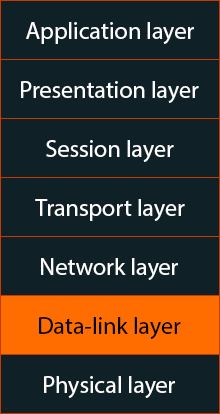
\includegraphics[width=0.25\textwidth]{images/osi.png}}
	\caption{Model OSI}
	\label{fig:osi}
\end{figure}

Stos protokołów LTE można odnieść do wszystkich siedmiu warstw modelu OSI (ISO Open Systems Interconnection Reference Model, Rys. \ref{fig:osi}). Model OSI jest traktowany jako model odniesienia dla większości rodzin protokołów komunikacyjnych. Podstawowym założeniem modelu jest podział systemów sieciowych na 7 warstw współpracujących ze sobą w ściśle określony sposób. \cite{Wiki01} Model OSI definiuje następujące 7 warstw:

\begin{enumerate}
	\item Warstwa aplikacji - odpowiada za udostępnianie interfejsu z którego korzystają aplikacje przestrzeni użytkownika
	\item Warstwa prezentacji - ma za zadanie przetworzenie danych z warstwy aplikacji do postaci kanonicznej, zgodnej ze specyfikacją OSI-RM
	\item Warstwa sesji - pozwala na stworzenie i utrzymanie sesji w ramach połączenia pomiędzy dwoma urządzeniami
	\item Warstwa transportowa - odbiera dane z wyższych warstw, dzieli na mniejsze fragmenty i dostarcza do niższych warstw. Odpowiada również za korekcję błędów
	\item Warstwa sieciowa - posiada wiedzę na temat topologi sieci i odpowiada za wytyczenie odpowiedniej trasy od nadawcy do odbiorcy
	\item Warstwa łącza danych - ma za zadanie obsługę błędów transmisji z warstwy fizycznej tak aby nie wpływały one na wyższe warstwy
	\item Warstwa fizyczna - odpowiada za przesyłanie bitów danych przez kanał komunikacyjny
\end{enumerate}

W tej pracy oraz w przygotowanej symulacji skupiono się na protokołach odpowiadającym warstwie 2. modelu OSI tj. warstwie łącza danych (Rys. \ref{fig:osi_to_lte}). LTE wyróżnia 3 podwarstwy (przedstawione po prawej stronie Rys. \ref{fig:osi_to_lte}) w obrębie warstwy 2. modelu OSI. Są to:

\begin{enumerate}
	\item Podwarstwa Packet Data Convergence Protocol (PDCP) - odpowiadająca za kwestię bezpieczeństwa transferu danych, kompresji nagłówków IP i stabilne dostarczanie pakietów podczas przełączanie urządzenia użytkownika pomiędzy stacjami bazowymi
	\item Podwarstwa Radio Link Control (RLC) - odpowiada za zapewnienie prawidłowego dostarczenia pakietów, których warstwa fizyczna nie była w stanie dostarczyć, poprzez ich ponowną retransmisję
	\item Podwarstwa Medium Access Control (MAC) - zarządza transmisją pakietów w czasie, steruje zachowaniem warstwy fizycznej
\end{enumerate}

Na Rys. \ref{fig:ip_through_layers} pokazano w ogólny sposób jak przykładowe pakiety IP są modyfikowane przez poszczególne podwarstwy warstwy 2. zanim zostaną dostarczone do warstwy fizycznej. Możemy tutaj zobaczyć jak pakiet IP odebrany z warstwy sieciowej, trafia do podwarstwy PDCP gdzie jest szyfrowany, jego nagłówek jest kompresowany i dodawany jest nagłówek podwarstwy PDCP. Proces ten dokladniej opisano w rozdziale \ref{cha:pdcp}. Następnie, w podwarstwie RLC, otrzymany pakiet jest dzielony na mniejsze fragmenty lub łączony z innymi (w zależności od potrzeb) i dodawany jest nagłówek podwarstwy RLC. Dokładny opis tego procesu zawarto w rozdziale \ref{cha:rlc}. Ostatnia podwarstwa - MAC - w razie konieczności łączy kilka jednostek danych z wyższej warstwy w jeden blok transportowy, dodaje swój nagłówek i przekazuje do warstwy fizycznej (rozdział \ref{cha:mac}).

\begin{figure}
	\centerline{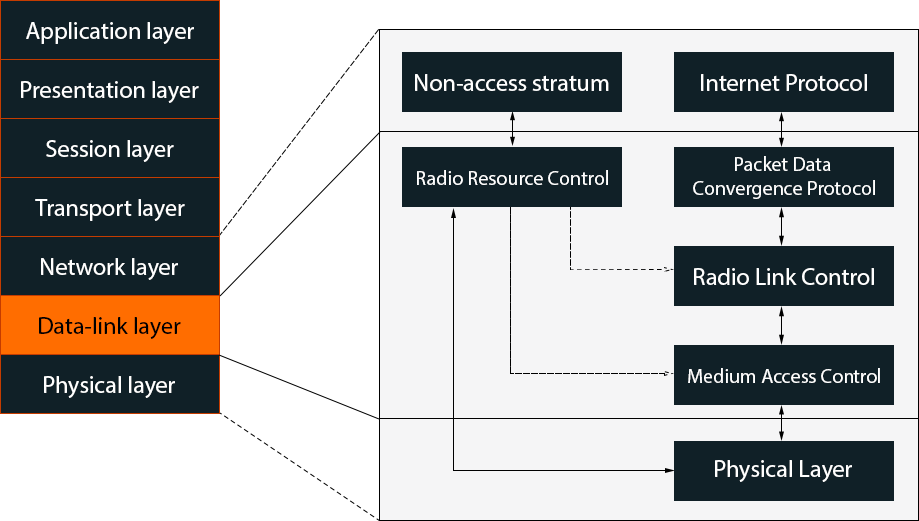
\includegraphics[width=1.0\textwidth]{images/osi_to_lte.png}}
	\caption{Implementacja warstwy 2. modelu OSI w LTE}
	\label{fig:osi_to_lte}
\end{figure}

\begin{figure}
	\centerline{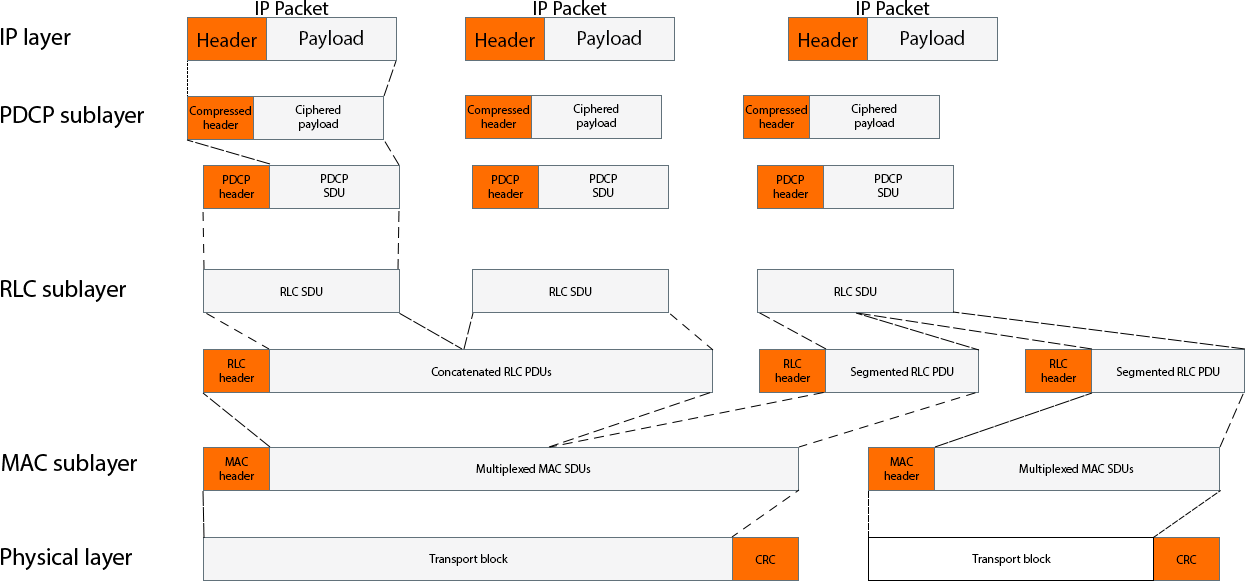
\includegraphics[width=1.0\textwidth]{images/pdu_overview.png}}
	\caption{Przetwarzanie pakietu IP na poszczegółnych podwarstwach warstwy 2.}
	\label{fig:ip_through_layers}
\end{figure}